\chapter{빛원뿔, 측지선, 슈바르츠실트 지평선}

지평선 문제는 특수상대성이론에 이미 존재하는 구분에서 출발한다. 서로 가까운 두 사건은 시간꼴, 공간꼴 또는 빛꼴 방향으로 분리될 수 있다. 곡률이 생겨도 이 분류가 사라지는 것은 아니다. 빛원뿔이 사건마다 다른 국소적인 대상이 되고, 계량 자체가 동역학적으로 변한다. 계량을 알면 자유낙하 입자의 운동은 평탄한 시공간에서 자유로운 상대론적 입자의 운동을 기술하는 것과 같은 고유시간 원리로부터 결정된다.

이 원리를 두 번 적용할 것이다. 먼저 약한 장에서 뉴턴 운동을 재현해야 한다. 그런 다음 시간, 방사 거리, 속도의 의미가 뜻밖에도 미묘해지는 슈바르츠실트 계량에 적용한다.

\section{시간꼴, 공간꼴, 빛꼴 간격}

평탄한 시공간에서 \(c=1\)일 때 고유시간 요소는 다음과 같다.
\begin{equation}
d\tau^2=dt^2-dx^2-dy^2-dz^2.
\label{eq:l5-minkowski-proper-time}
\end{equation}
비상대론적 근사가 적용될 만한 상황에서는 \(c\)를 다시 포함해 쓰면 편리하다.
\begin{equation}
d\tau^2
=dt^2-\frac{dx^2+dy^2+dz^2}{c^2}.
\label{eq:l5-minkowski-c}
\end{equation}
\(d\tau^2\)라는 표기만으로 우변이 양수임을 보장할 수는 없다. 그 부호로 변위를 분류한다.
\begin{align}
d\tau^2>0
&\quad\Longleftrightarrow\quad \text{time-like},\\
d\tau^2=0
&\quad\Longleftrightarrow\quad \text{light-like},\\
d\tau^2<0
&\quad\Longleftrightarrow\quad \text{space-like}.
\end{align}
공간꼴 변위에 대해서는 양의 고유거리를 정의하는 것이 편리하다.
\begin{equation}
ds^2=-d\tau^2
=dx^2+dy^2+dz^2-dt^2
\qquad(c=1).
\label{eq:l5-proper-distance}
\end{equation}

빛원뿔은 이 세 가지 가능성을 체계화한다. 빛꼴 방향은 원뿔의 내부가 아니라 표면을 이룬다. 시간꼴 방향은 원뿔 안쪽에, 공간꼴 방향은 바깥쪽에 놓인다. 위쪽과 아래쪽 절반은 각각 미래와 과거의 빛원뿔을 나타낸다.

\begin{figure}[htbp]
\centering
\includegraphics[width=0.82\textwidth]{lecture_05_figure_02.png}
\caption{칠판에 함께 나타낸 고유시간, 고유거리, 인과 원뿔. 빛살은 원뿔 자체를 이루며, 내부는 시간꼴이고 외부는 공간꼴이다.}
\lectureframe{00:05:44}
\end{figure}

\begin{figure}[htbp]
\centering
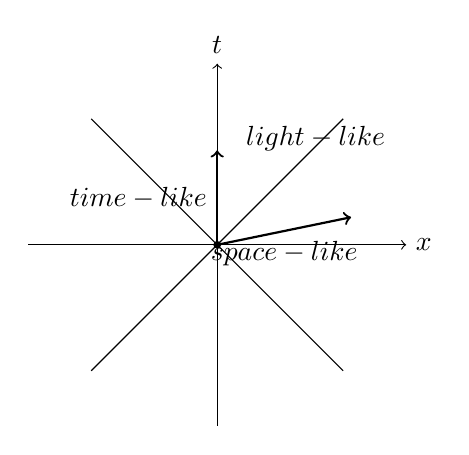
\begin{tikzpicture}[scale=1.0]
\draw[->] (0,-2.3) -- (0,2.3) node[above] {\(t\)};
\draw[->] (-2.4,0) -- (2.4,0) node[right] {\(x\)};
\draw (-1.6,1.6) -- (0,0) -- (1.6,1.6);
\draw (-1.6,-1.6) -- (0,0) -- (1.6,-1.6);
\fill (0,0) circle (1.4pt);
\draw[->,thick] (0,0) -- (0,1.2)
  node[midway,left] {\(\text{time-like}\)};
\draw[->,thick] (0,0) -- (1.7,0.35)
  node[midway,below] {\(\text{space-like}\)};
\node at (1.25,1.35) {\(\text{light-like}\)};
\end{tikzpicture}
\caption{2차원 시공간 단면에서의 인과적 분류.}
\end{figure}

이 간격들은 실제 측정과 관련된다. 고유시간은 시간꼴 세계선에 따라 운반되는 시계가 가리키는 시간이다. 고유거리는 공간꼴로 분리된 사건들 사이에서 적절한 자 세트가 측정하는 거리다. 이는 단지 이차 형식의 부호에 붙인 이름이 아니다.

\section{로런츠 부호수와 사건마다 놓인 원뿔}

주로 양의 부호를 쓰는 텐서 관례를 사용하면 평탄 계량의 성분은 다음과 같다.
\begin{equation}
\eta_{\mu\nu}=\operatorname{diag}(-1,1,1,1),
\label{eq:l5-eta}
\end{equation}
그리고
\begin{equation}
d\tau^2=-\eta_{\mu\nu}\,dx^\mu dx^\nu.
\label{eq:l5-proper-time-eta}
\end{equation}
표시된 행렬은 특히 단순한 한 기저에서 표현한 2계 텐서다. 불변적인 특징은 그 부호수, 즉 음의 방향 하나와 양의 방향 셋이다.
\begin{equation}
\operatorname{signature}(\eta)=(-,+,+,+).
\label{eq:l5-lorentz-signature}
\end{equation}
음의 부호가 두 개인 계량은 시간 방향이 둘인 경우에 해당한다. 그런 부호수도 수학적으로 연구할 수 있지만, 여기서 가정하는 시공간을 기술하지는 않는다.

곡선 시공간에서는 성분이 위치에 따라 변한다.
\begin{equation}
g_{\mu\nu}=g_{\mu\nu}(x).
\label{eq:l5-position-metric}
\end{equation}
각 사건에서 계량은 여전히 로런츠 부호수를 가져야 한다. 따라서 각 사건에는 그 사건에 고유한 시간꼴 방향, 빛꼴 경계, 공간꼴 방향이 있다. 좌표 그림에서는 원뿔이 지점마다 기울거나 납작해 보일 수 있지만, 인과적 분류는 그대로 유지된다.

\begin{figure}[htbp]
\centering
\includegraphics[width=0.86\textwidth]{lecture_05_figure_03.png}
\caption{위치에 따라 달라지는 계량 \(g_{\mu\nu}(x)\), 인과적 분류, 국소 빛원뿔의 그림.}
\lectureframe{00:09:41}
\end{figure}

\begin{figure}[htbp]
\centering
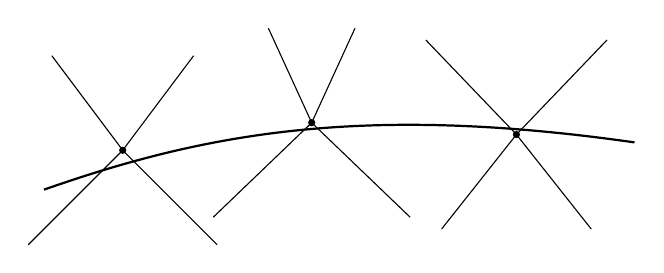
\begin{tikzpicture}[scale=1.0]
\draw[thick] (-4,-0.5) .. controls (-2,0.2) and (0,0.6) .. (3.5,0.1);
\foreach \x/\y/\a/\b in {-3/0/0.9/1.2, -0.6/0.35/0.55/1.25,
                          2.0/0.2/1.15/0.95} {
  \fill (\x,\y) circle (1.3pt);
  \draw (\x,\y) -- ++(-\a,1.2);
  \draw (\x,\y) -- ++(\a,1.2);
  \draw (\x,\y) -- ++(-\b,-1.2);
  \draw (\x,\y) -- ++(\b,-1.2);
}
\end{tikzpicture}
\caption{이웃한 국소 원뿔들. 좌표상 모양은 달라질 수 있지만, 어떤 벡터가 시간꼴, 빛꼴, 공간꼴인지는 바뀌지 않는다.}
\end{figure}

\begin{classroomqa}
\audiencequestion{음의 고윳값 하나가 유일한 시간 방향을 정하는가?}
\lecturerresponse{표시된 행렬을 대각화하는 기저에는 음의 기저 방향이 하나 있지만, 그것이 선호되는 관측자나 유일한 물리적 시간 방향을 정해 주지는 않는다. 로런츠 변환은 시간 좌표와 공간 좌표를 서로 섞으며, 원뿔 안의 모든 벡터는 시간꼴이다. 불변적인 대상은 특정한 시간꼴 벡터 하나가 아니라, 원뿔과 음의 부호 하나·양의 부호 셋이라는 부호수다.
\lecturetimestamp{00:12:17--00:17:24}}
\end{classroomqa}

\begin{classroomqa}
\audiencequestion{국소 원뿔을 그린 두 그림의 모양은 왜 다를 수 있는가?}
\lecturerresponse{좌표에 따라 그림이 달라질 수 있다. 예를 들어 \(x\)를 크기가 재조정된 좌표로 바꾸면 빛살에 부여되는 수치상의 기울기가 달라져 원뿔이 더 좁거나 넓어 보인다. 더 일반적인 좌표 변환은 원뿔을 기울게 할 수도 있다. 두 그림은 같은 사건과 같은 인과 관계를 나타낸다. 곡선 시공간에서는 서로 다른 사건의 원뿔이 서로 다른 접공간에 속하므로, 이들을 비교하려면 계량과 평행이동 규칙이 필요하다.
\lecturetimestamp{00:13:37--00:15:59}}
\end{classroomqa}

\section{변분 문제로서의 측지선}

자유롭게 움직이는 입자는 시공간 측지선을 따른다. 아핀 매개변수 \(\lambda\)를 사용해 미분형으로 쓰면 다음과 같다.
\begin{equation}
\frac{d^2x^\mu}{d\lambda^2}
+\Gamma^\mu{}_{\rho\sigma}
\frac{dx^\rho}{d\lambda}
\frac{dx^\sigma}{d\lambda}=0.
\label{eq:l5-geodesic}
\end{equation}
접속은 입자가 움직일 때 접벡터가 자기 자신과 평행을 유지하도록 하는 역할을 한다.

계산에는 두 번째 정식화가 더 편리한 경우가 많다. 계량 \(g_{mn}\)을 갖는 리만 공간에서 곡선의 길이는 다음과 같다.
\begin{equation}
s=\int ds
=\int\sqrt{g_{mn}\,dx^m dx^n}.
\label{eq:l5-spatial-length}
\end{equation}
측지선은 양 끝점을 고정한 채 경로를 조금씩 변분했을 때 이 길이가 정지값을 갖는 곡선이다. 적분은 곡선을 따라 미소 길이를 단순히 합한 것이며, 오일러--라그랑주 방정식은 힘의 법칙과 형태가 유사한 2계 미분방정식이다.

시간꼴 세계선에서는 공간 길이 대신 고유시간을 사용한다.
\begin{equation}
\tau
=\int\sqrt{-g_{\mu\nu}\,dx^\mu dx^\nu}.
\label{eq:l5-proper-time-functional}
\end{equation}
시간꼴 측지선에서는 \(\tau\)가 정지값을 가지며, 공액점이 생기기 전의 가까운 자유낙하 경로들 사이에서는 국소 최댓값이 된다. 여기에 \(-m\)를 곱하면 입자의 작용이 된다.
\begin{equation}
A=-m\tau
=-m\int\sqrt{-g_{\mu\nu}\,dx^\mu dx^\nu}.
\label{eq:l5-particle-action}
\end{equation}
따라서 같은 경로가 \(A=-m\tau\)를 국소적으로 최소화한다. 고유시간이 정지값을 갖는다는 사실과 작용에 선택한 부호를 구분하면 최소와 최대가 서로 모순되는 듯한 문제는 해소된다.

\section{고유시간에서 통상적인 라그랑지안으로}

\eqref{eq:l5-particle-action}의 작용은 기하학적이지만, 역학에서 익숙하게 쓰는 형태로 바꿀 수 있다. 세계선을 좌표 \(t\)로 매개화하고, 각 미분을 \(dt\)로 나눈 뒤 남은 \(dt\) 인자를 제곱근 바깥으로 빼면 다음과 같다.
\begin{align}
A
&=-m\int\sqrt{-g_{\mu\nu}(x)\,dx^\mu dx^\nu}\\
&=-m\int
\sqrt{-g_{\mu\nu}(x)
\frac{dx^\mu}{dt}\frac{dx^\nu}{dt}}\,dt.
\label{eq:l5-action-t}
\end{align}
시간 성분에 대해서는 \(dt/dt=1\)이고, 공간 성분은 통상적인 좌표 속도다. 따라서 다음과 같이 쓸 수 있다.
\begin{equation}
\begin{aligned}
A&=\int L\,dt,\\
L&=-m\sqrt{-g_{\mu\nu}(x)\dot x^\mu\dot x^\nu},\\
\dot x^\mu&=\frac{dx^\mu}{dt}.
\end{aligned}
\label{eq:l5-relativistic-lagrangian}
\end{equation}

\begin{figure}[htbp]
\centering
\includegraphics[width=0.88\textwidth]{lecture_05_figure_05.png}
\caption{세계선 작용을 통상적인 형태 \(A=\int L\,dt\)로 바꾸는 과정.}
\lectureframe{00:27:00}
\end{figure}

\begin{figure}[htbp]
\centering
\includegraphics[width=0.88\textwidth]{lecture_05_figure_06.png}
\caption{상대론적 라그랑지안만 남도록 정리한 뒤의 칠판 상태.}
\lectureframe{00:28:59}
\end{figure}

\begin{classroomqa}
\audiencequestion{이 작용에서 시공간 지표는 그리스 문자로 써야 하는가?}
\lecturerresponse{그렇다. 그리스 지표는 시간 좌표와 모든 공간 좌표에 걸쳐 돈다. 구분이 유용할 때는 공간 좌표에 라틴 지표를 사용할 수 있다.
\lecturetimestamp{00:25:53--00:26:03}}
\end{classroomqa}

\begin{classroomqa}
\audiencequestion{제곱근 형태의 식을 왜 라그랑지안이라고 부르는가?}
\lecturerresponse{작용을 \(A=\int L\,dt\)로 쓰고 나면 그 피적분함수가 라그랑지안이다. 이는 단순한 정의에 그치지 않는다. 이 피적분함수를 변분하면 오일러--라그랑주 방정식이 나오며,
\[
\frac{d}{dt}
\left(\frac{\partial L}{\partial\dot x^\mu}\right)
=\frac{\partial L}{\partial x^\mu},
\]
매개변수를 일관되게 다루면 이 방정식은 측지선 방정식과 동등하다.
\lecturetimestamp{00:28:36--00:29:02}}
\end{classroomqa}

질량이 있는 입자의 세계선은 시간꼴이므로 제곱근 안의 양은 양수다. 공간꼴 경로는 보통의 질량을 가진 입자의 궤적이 아니라 초광속 운동을 나타낸다. 계량이 주어지면 크리스토펠 기호를 계산해 \eqref{eq:l5-geodesic}를 사용하거나, 오일러--라그랑주 방정식을 \eqref{eq:l5-relativistic-lagrangian}에 적용해 입자의 경로를 구할 수 있다. 두 방법이 동등함을 보이는 것은 유익한 연습이며, 보통은 작용을 이용하는 편이 더 간단하다.

\section{뉴턴 극한}

구형 질량원 바깥의 약하고 정적인 중력장을 생각하자. 평탄한 시공간에서 출발해 \(dt^2\)의 계수가 1에서 조금 벗어나도록 둔다.
\begin{equation}
d\tau^2
=\left(1+\frac{2u(\mathbf{x})}{c^2}\right)dt^2
-\frac{d\mathbf{x}^2}{c^2},
\label{eq:l5-weak-metric}
\end{equation}
여기서 \(u\)는 뉴턴 퍼텐셜이 될 양이다. 이 가정은 이름만 붙일 것이 아니라 검증해야 한다.

질량을 포함한 작용은 다음과 같다.
\begin{equation}
A=-mc^2\int
\sqrt{1+\frac{2u}{c^2}
-\frac{\dot{\mathbf{x}}^{\,2}}{c^2}}\,dt.
\label{eq:l5-weak-action}
\end{equation}
\(u/c^2\)와 \(\dot{\mathbf{x}}^{\,2}/c^2\)는 모두 작다. 1차 기여까지 남기면
\begin{equation}
\sqrt{1+\epsilon}
=1+\frac{\epsilon}{2}+O(\epsilon^2),
\qquad
\epsilon=\frac{2u-\dot{\mathbf{x}}^{\,2}}{c^2},
\end{equation}
다음 식을 얻는다.
\begin{align}
L
&=-mc^2
\sqrt{1+\frac{2u-\dot{\mathbf{x}}^{\,2}}{c^2}}\\
&=-mc^2-mu+\frac{m}{2}\dot{\mathbf{x}}^{\,2}\\
&\quad+O\!\left(c^{-2}
 [u^2+u\dot{\mathbf{x}}^{\,2}+\dot{\mathbf{x}}^{\,4}]\right).
\label{eq:l5-newton-expansion}
\end{align}
정지 에너지 상수항은 운동방정식에 영향을 주지 않는다. 남는 것은
\begin{equation}
L_{\mathrm{nr}}
=\frac{m}{2}\dot{\mathbf{x}}^{\,2}-m u(\mathbf{x}),
\label{eq:l5-newton-lagrangian}
\end{equation}
이므로 다음과 같다.
\begin{equation}
m\ddot{\mathbf{x}}=-m\boldsymbol{\nabla}u.
\label{eq:l5-newton-equation}
\end{equation}
시험 질량은 소거된다. 그래야 보편적 자유낙하와 일치한다. 퍼텐셜 에너지는 \(m u\)이고, 가속도는 \(m\)와 무관하다.

따라서 약한 장에서 성립하는 선도 관계를 다음과 같이 확인했다.
\begin{equation}
g_{00}=1+\frac{2u}{c^2}+O(c^{-4}).
\label{eq:l5-g00-newton}
\end{equation}
구형 질량 \(M\)의 바깥에서는
\begin{equation}
u(r)=-\frac{GM}{r},
\qquad
g_{00}=1-\frac{2GM}{rc^2}+O(c^{-4}).
\label{eq:l5-g00-spherical}
\end{equation}
이로써 시간 성분의 첫 번째 보정항이 결정된다. 하지만 강한 장 계량 전체가 결정된 것은 아니다.

\section{구면좌표와 첫 번째 슈바르츠실트 추정}

중심 질량원에는 구면좌표가 자연스럽다. 이 강의에서는 \(\theta\)를 극이 아니라 적도면에서부터 재므로, 각도 선요소는 다음과 같다.
\begin{equation}
d\Omega^2=d\theta^2+\cos^2\theta\,d\phi^2.
\label{eq:l5-angular-metric}
\end{equation}
이 관례를 따르면
\begin{equation}
d\mathbf{x}^2=dr^2+r^2d\Omega^2.
\label{eq:l5-flat-spherical}
\end{equation}
\(\theta\)처럼 위도에 해당하는 각을 택해도 물리량에는 아무런 영향이 없다. 더 흔히 쓰는 극각을 사용하면 \(\cos^2\theta\) 대신
\(\sin^2\theta\)가 들어간다.

공간 계량은 평탄한 채로 두고 뉴턴 극한에서 얻은 시간 계수를 대입하면 첫 번째 추정식은 다음과 같다.
\begin{equation}
\begin{aligned}
d\tau^2
&=\left(1-\frac{r_s}{r}\right)dt^2
-\frac{1}{c^2}\left(dr^2+r^2d\Omega^2\right),\\
r_s&=\frac{2GM}{c^2}.
\end{aligned}
\label{eq:l5-naive-schwarzschild}
\end{equation}
이 식은 정확한 답일 수 없다. \(r<r_s\)에서는 \(dt^2\)의 계수 부호가 바뀌지만, 고유시간 관례에서 모든 공간 계수는 음수로 남는다. 그러면 계량은 시간 방향 하나와 공간 방향 셋으로 이루어진 부호수를 잃는다.

진공 장방정식으로부터 필요한 방사 계수를 얻는다.
\begin{equation}
\boxed{
d\tau^2
=\left(1-\frac{r_s}{r}\right)dt^2
-\frac{dr^2}{c^2\left(1-r_s/r\right)}
-\frac{r^2}{c^2}d\Omega^2.
}
\label{eq:l5-schwarzschild}
\end{equation}
이것이 외부 슈바르츠실트 계량이다. \(r\)가 \(r_s\)를 지나면 \(t\)와 \(r\)의 계수가 함께 부호를 바꾸어 로런츠 부호수가 보존된다. 슈바르츠실트 좌표에서는 내부에서 방사 좌표가 시간꼴이 되고 좌표 \(t\)가 공간꼴이 된다. 이러한 교환은 지평선에서 좌표 도표가 실패한다는 뜻이지, 시공간 기하 자체가 국소적으로 실패한다는 뜻은 아니다.

\begin{classroomqa}
\audiencequestion{낙하하는 물체가 지평선을 통과하는 데 얼마나 걸리는가?}
\lecturerresponse{먼 거리 관측자가 사용하는 슈바르츠실트 좌표 시간 \(t\)으로 측정하면 통과 시각은 무한대로 밀려난다. 낙하하는 물체의 시계가 재는 고유시간으로는 유한한 시간 안에 통과한다. 이 시계들 사이의 차이가 지평선을 둘러싼 핵심적인 수수께끼다.
\lecturetimestamp{00:54:45--00:55:35}}
\end{classroomqa}

\begin{classroomqa}
\audiencequestion{다른 계량 성분이 아니라 방사 계수를 바꾸는 이유는 무엇인가?}
\lecturerresponse{계량은 로런츠 부호수를 유지해야 하고, 구면대칭에서는 방사 방향이 각도 방향의 구면과 구별되며, 진공 장방정식은 정확한 역수 인자를 결정한다. 부호수는 어느 부분을 살펴봐야 할지 알려 줄 뿐이고, 정확한 결과는 아인슈타인 방정식이 준다.
\lecturetimestamp{00:55:35--00:56:01}}
\end{classroomqa}

지구의 경우 \(r_s\)는 물질로 이루어진 천체 내부 깊숙한 곳에 있으며, 그 크기는 겨우 센티미터 정도다. 그곳에서는 외부 진공 계량이 유효하지 않으므로 지구에는 슈바르츠실트 지평선이 없다. 물질 내부에서는 내부 해로 대체하고, 표면에서 외부 해와 이어 맞춰야 한다.

\begin{classroomqa}
\audiencequestion{\(t\)와 \(r\)가 좌표 역할을 서로 바꾼다면 보통 시계에는 무슨 일이 생기는가?}
\lecturerresponse{시계는 시간꼴 세계선을 따라 고유시간을 계속 측정한다. 선택한 좌표가 다루기 까다로워졌다는 사실은 시계에 영향을 주지 않는다. 정칙적인 자유낙하 좌표계를 사용하면 지평선을 지나는 국소 기하와 보통의 국소 빛 전파가 매끄럽다는 점을 확인할 수 있다.
\lecturetimestamp{00:56:35--00:57:50}}
\end{classroomqa}

\subsection{방사 보정항이 뉴턴 운동방정식에 나타나지 않는 이유}

정확한 계량에서는 퍼텐셜의 1차에서 이미 방사 계수가 변한다.
\begin{equation}
\frac{1}{1-r_s/r}
=1+\frac{r_s}{r}
+O\!\left(\frac{r_s^2}{r^2}\right)
=1-\frac{2u}{c^2}+O(c^{-4}).
\label{eq:l5-radial-expansion}
\end{equation}
뉴턴 유도 과정에서 이 변화를 무시해도 되는 이유는 무엇일까? 입자 작용 안에서 이 항은 \(\dot r^2/c^2\)를 곱한다. 따라서 그 1차 보정은
\begin{equation}
\frac{u\,\dot r^2}{c^4},
\end{equation}
에 비례하며, 이는 \eqref{eq:l5-newton-expansion}에서 남긴 차수를 넘는다. 느린 운동의 뉴턴 근사 시험에서는 방사 보정항이 무시해도 될 만큼 작지만, 상대론적 운동과 지평선 부근에서는 결정적인 역할을 한다. 한 근사에서는 너무 작아 무시되는 항이 다른 근사에서는 관심 현상을 좌우할 수 있다는 점을 기억해야 한다.

\section{슈바르츠실트 시간에서의 방사 낙하}

\(c=1\)로 두고 먼저 방사 운동을 살펴보자. 원운동도 중요하지만 각도 항이 필요하므로 뒤에서 다룬다. 방사 운동은 궤도 운동이라기보다 중심 질량원 쪽으로 곧장 추락하는 운동에 가깝고, 계산이 가장 간단해 지평선에서의 거동을 드러내 준다.

\begin{classroomqa}
\audiencequestion{방사 속도에 나타나는 시간은 누구의 시간인가?}
\lecturerresponse{아래 점은 먼 거리의 정지 관측자에 맞춰 정규화한 슈바르츠실트 좌표 시간 \(t\)에 대한 미분을 뜻한다. 낙하하는 관측자의 손목시계는 고유시간 \(\tau\)을 잰다. 둘을 혼동하면 좌표에 관한 진술을 잘못된 국소적 진술로 바꾸게 된다.
\lecturetimestamp{01:04:03--01:04:47}}
\end{classroomqa}

\(d\Omega=0\)일 때 다음을 정의하자.
\begin{equation}
a(r)=1-\frac{r_s}{r}.
\label{eq:l5-a-def}
\end{equation}
방사 계량과 라그랑지안은 다음과 같다.
\begin{align}
d\tau^2&=a\,dt^2-\frac{dr^2}{a},\\
L&=-m\sqrt{a-\frac{\dot r^2}{a}},
\qquad
\dot r=\frac{dr}{dt}.
\label{eq:l5-radial-lagrangian}
\end{align}
\(L\)은 \(t\)에 명시적으로 의존하지 않으므로 해밀토니안은 보존된다. 방사 운동량은
\begin{equation}
p_r=\frac{\partial L}{\partial\dot r}
=\frac{m\dot r}{a\sqrt{a-\dot r^2/a}},
\label{eq:l5-radial-momentum}
\end{equation}
이고,
\begin{align}
H
&=p_r\dot r-L\\
&=\frac{ma}{\sqrt{a-\dot r^2/a}}
=E.
\label{eq:l5-radial-energy}
\end{align}
좌표 속도를 풀어 쓰면 다음과 같다.
\begin{equation}
\boxed{
\dot r^2
=a^2\left(1-\frac{m^2}{E^2}a\right).
}
\label{eq:l5-radial-velocity}
\end{equation}
칠판 계산에서는 몇 가지 중간 대수식을 검토하며, 상자 안의 식이 일관된 결과다.

\(r\)가 \(r_s\)에 가까워질수록 \(a(r)\)는 0에 가까워지고 괄호 안의 인자는 1에 가까워진다. 따라서 유입하는 입자에 대해서는
\begin{equation}
\frac{dr}{dt}
\sim -\left(1-\frac{r_s}{r}\right)
\longrightarrow 0
\qquad(r\longrightarrow r_s^+)
\label{eq:l5-infall-freeze}
\end{equation}
이 된다. 슈바르츠실트 시간으로 보면 입자는 지평선 바로 바깥에서 점점 느려져 멈춘 것처럼 보인다.

\begin{classroomqa}
\audiencequestion{\(dr/dt\) 값이 감소한다는 것은 중력이 반발력으로 바뀌었다는 뜻인가?}
\lecturerresponse{아니다. 입자가 국소적으로 바깥쪽으로 밀리는 것은 아니다. 좌표 \(t\)는 통과 과정을 기술하기에 점점 부적절해지므로, 단위 \(t\)당 방사 방향 진행량이 0에 가까워진다. 자유낙하 세계선을 따른 고유가속도는 계속 0이며, 지평선은 유한한 고유시간 안에 도달한다.
\lecturetimestamp{01:14:18--01:16:38}}
\end{classroomqa}

실제로 지평선 근처에서는
\begin{equation}
\frac{dt}{dr}
\sim-\frac{1}{1-r_s/r}
=-\frac{r}{r-r_s}.
\end{equation}
이 된다. 이를 적분하면 로그 발산이 생긴다. 이는 낙하하는 물체의 시계가 무한한 시간을 가리킨다는 뜻이 아니라, 슈바르츠실트 시간으로 측정한 통과 시간이 무한하다는 점을 증명한다.

\section{방사 방향 빛살}

빛의 경우 같은 계산을 가장 짧게 할 수 있다. 방사 방향 영측지선에서는
\begin{equation}
d\tau^2
=a\,dt^2-\frac{dr^2}{a}=0.
\end{equation}
따라서
\begin{equation}
\boxed{
\frac{dr}{dt}
=\pm a(r)
=\pm\left(1-\frac{r_s}{r}\right).
}
\label{eq:l5-radial-light}
\end{equation}
가 된다. 양의 부호는 바깥쪽으로 나가는 빛살을, 음의 부호는 안쪽으로 들어오는 빛살을 나타낸다. 두 빛살 모두 좌표 속도는 지평선에서 0에 가까워진다.

\begin{classroomqa}
\audiencequestion{중심 질량원에서 멀리 떨어진 곳에서는 이 식이 어떤 속도를 주는가?}
\lecturerresponse{\(r\)가 무한대로 갈 때 \(a(r)\)는 1에 가까워지므로 \(dr/dt\)는 \(\pm1\), 즉 단위를 복원하면 \(\pm c\)에 가까워진다.
\lecturetimestamp{01:21:01--01:21:29}}
\end{classroomqa}

일반상대성이론에서는 이런 일이 흔하다. 원리는 몇 줄이면 충분하지만 좌표와 계산은 복잡해진다. 방정식 \eqref{eq:l5-radial-light}는 간단하지만, \(r_s\) 부근에서 그 값이 사라지는 것을 해석할 때는 주의가 필요하다. 이는 좌표 속도이지 국소 관성 관측자가 측정하는 속도가 아니다.

\section{먼 거리 관측자에게 보이는 것}

\begin{classroomqa}
\audiencequestion{지평선 부근에서 방출된 빛은 탈출할 수 있는가? 이것이 호킹 복사인가?}
\lecturerresponse{지평선 바로 바깥에서 방출된 고전적 바깥방향 빛살은 바깥으로 움직일 수 있지만, 그 슈바르츠실트 좌표 속도는 극히 작은 값에서 출발하며 신호가 무한대에 도달하기까지 큰 지연과 적색편이를 겪는다. 지평선 위의 빛살은 이 좌표계에서 지평선 위에 머물고, 내부의 빛살은 탈출할 수 없다. 호킹 복사는 외부 기하와 관련된 양자장 효과이지 내부에서 빠져나오는 고전적 빛살이 아니며, 여기서 수행한 계산으로 유도되는 현상도 아니다.
\lecturetimestamp{01:22:08--01:24:28}}
\end{classroomqa}

\begin{classroomqa}
\audiencequestion{광자가 거의 정지한 것처럼 보이면 질량이 있는 것처럼 보이기 시작하는가?}
\lecturerresponse{아니다. 자유낙하하는 국소 관측자는 언제나 광자의 속도를 \(c\)로 측정한다. 0에 가까워지는 것은 좌표 비율 \(dr/dt\)뿐이다. 나쁜 좌표 도표가 질량이나 영성, 국소 광속을 바꾸지는 않는다.
\lecturetimestamp{01:24:31--01:25:26}}
\end{classroomqa}

여기서 사용한 슈바르츠실트 해는 외부 진공 해다. 별, 행성 또는 붕괴하는 구름에는 이 해와 접합해야 하는 다른 내부 계량이 있다. 지구처럼 물질 표면이 \(r_s\) 바깥에 큰 차이로 머물러 있다면, 진공 공식으로 정의되는 외부 좌표 지평선은 물질을 통과해 진공 해를 연장할 수 있는 영역 밖에 놓인다. 천체가 슈바르츠실트 반지름 안쪽으로 붕괴하면 지평선은 물리적 시공간의 일부가 된다.

\begin{classroomqa}
\audiencequestion{외부 관측자가 물질이 통과하는 모습을 끝내 보지 못한다면, 블랙홀은 어떻게 생기거나 성장할 수 있는가?}
\lecturerresponse{이 전제는 슈바르츠실트 시간을 지평선에서 통용되는 전역적 물리 시계인 것처럼 취급한다. 따라서 블랙홀이 결코 성장할 수 없다는 결론은 그럴듯해 보이지만 틀렸다. 완전한 답을 얻으려면 지평선을 매끄럽게 통과하는 좌표와 붕괴의 전역적 인과 기하가 필요하며, 그 문제의 해명은 강의의 다음 단계로 미룬다.
\lecturetimestamp{01:27:57--01:29:36}}
\end{classroomqa}

\begin{classroomqa}
\audiencequestion{지평선으로 떨어지는 자동차를 레이더 속도계로 측정하면 어떤 값이 나오는가?}
\lecturerresponse{좌표 속도는 자동차가 떨어지는 동안 먼저 증가하다가 방향을 바꿔 0을 향해 감소한다. 나중에 보낸 레이더 펄스도 지평선 바깥에 있는 자동차를 따라잡을 수 있지만, 왕복 시간은 점점 길어진다. 되돌아오는 신호는 점점 더 적색편이되고, \(r_s\) 부근에서 영상은 느려지고 압축되어 보인다. 이것은 운전자가 실제로 경험하는 상황을 국소적으로 잘 나타내는 그림이 아니다. 운전자는 유한한 고유시간 안에 지평선을 통과한다.
\lecturetimestamp{01:29:39--01:32:14}}
\end{classroomqa}

\begin{classroomqa}
\audiencequestion{빛의 속도가 일정한 것은 특수상대성이론에서만인가?}
\lecturerresponse{일반상대성이론에서도 모든 국소 관성계에서 빛의 속도는 일정하다. 국소 시계와 자를 가지고 자유낙하하는 관측자는 가까운 광자의 속도를 \(c\)로 측정한다. \(dr/dt\)와 같은 좌표 속도는 변할 수 있는데, 이는 \(r\)와 \(t\)가 시공간 전체에 걸친 하나의 국소 관성 실험실에서 나온 측정값이 아니기 때문이다.
\lecturetimestamp{01:32:20--01:34:20}}
\end{classroomqa}

\section{슈바르츠실트 계산을 넘어서는 질문들}

\begin{classroomqa}
\audiencequestion{중력을 다른 힘들과 통일한다는 것은 무엇을 뜻할 수 있는가?}
\lecturerresponse{기하학적 가능성 가운데 하나는 추가적인 압축 차원을 더해 시공간을 확장하는 것이다. 그러면 고차원 계량의 성분이 4차원에서는 게이지 장과 스칼라 장으로 나타날 수 있고, 추가 차원 방향의 운동량은 전하처럼 나타날 수 있다. 이는 칼루차--클라인 구상과 관련된 구조적 단서이지, 이번 강의에서 완성된 통일 이론은 아니다.
\lecturetimestamp{01:34:22--01:36:08}}
\end{classroomqa}

\begin{classroomqa}
\audiencequestion{서로 다른 영역이나 우주에서 계량의 부호수가 다를 수 있는가?}
\lecturerresponse{고전 일반상대성이론에서는 보통 비퇴화 로런츠 부호수를 고정해 둔다. 부호수를 바꾸려면 계량이 퇴화된 배치를 거쳐야 하며, 그곳에서는 표준적인 고전적 기술이 성립하지 않는다. 양자중력은 더 포괄적인 언어를 요구할 수도 있지만, 물리적으로 부호수가 바뀌는 영역을 예측하는 확립된 이론은 여기서 제시되지 않는다.
\lecturetimestamp{01:36:08--01:38:08}}
\end{classroomqa}

\begin{classroomqa}
\audiencequestion{슈바르츠실트는 제1차 세계대전 중 복무하면서 어떻게 이 해를 찾았는가?}
\lecturerresponse{강의에서 강조한 점은 역사적일 뿐 아니라 인간적인 면도 있다. 슈바르츠실트는 천문학자이자 매우 뛰어난 수학자였으며, 아인슈타인의 새로운 방정식을 연구하는 일이 전시 복무 중 지적 피난처가 되어 주었다.
\lecturetimestamp{01:38:11--01:39:02}}
\end{classroomqa}

이제 핵심 교훈이 다음 단계로 이어갈 만큼 분명해졌다. 계량은 인과 원뿔과 자유 운동을 모두 결정한다. 약한 장에서 계량의 시간 성분에는 뉴턴 퍼텐셜이 들어 있고, 정확한 슈바르츠실트 계량은 \(r=r_s\)에 좌표 지평선을 둔다. 슈바르츠실트 시간으로 측정한 통과 시간은 무한대로 늘어나지만, 낙하 관측자의 고유시간은 그렇지 않다. 이 대비를 전역적으로 해명하고, 멀리서 얼어붙은 듯 보이는 영상에도 블랙홀이 형성되는 이유를 설명하는 것이 다음 문제다.